\documentclass{beamer}
\mode<presentation>{
  \usetheme{Boadilla}
  \usefonttheme[onlylarge]{structurebold}
  \usefonttheme[stillsansseriflarge]{serif}
  \setbeamerfont*{frametitle}{size=\normalsize,series=\bfseries}
  % \setbeamertemplate{navigation symbols}{}
  \setbeamercovered{transparent}
}
\usepackage[english]{babel}
\usepackage[latin1]{inputenc}
\usepackage{times}
\usepackage[T1]{fontenc}
\usepackage{amsmath}
\usepackage{amssymb}
\usepackage{esint}
\usepackage{hyperref}
\usepackage{tikz}
\usepackage{circuitikz}
\usepackage{xkeyval}
\usepackage{xargs}
\usepackage{xcolor}
\usepackage{verbatim}
\usepackage{listings}
\usepackage{multimedia}
\usepackage{bm}
\usepackage{siunitx}
\usetikzlibrary{
  arrows,
  calc,
  decorations.pathmorphing,
  decorations.pathreplacing,
  decorations.markings,
  fadings,
  positioning,
  shapes,
  arrows.meta
}
\usepgfmodule{oo}

\pgfdeclareradialshading{glow2}{\pgfpoint{0cm}{0cm}}{
  color(0mm)=(white);
  color(2mm)=(white);
  color(8mm)=(black);
  color(10mm)=(black)
}
\pgfdeclareradialshading{glow}{\pgfpoint{0cm}{0cm}}{
  color(0mm)=(white);
  color(5mm)=(white);
  color(9mm)=(black);
  color(10mm)=(black)
}
\pgfdeclareverticalshading{north edge}{2cm}{
  % manual 1082-1083; later - shading is assumed to be 100bp diameter ??
  color(0cm)=(white);
  color(1.3cm)=(white);
  color(1.5cm)=(black)
}

\begin{tikzfadingfrompicture}[name=glow fading]
  \shade [shading=glow] (0,0) circle (1);
\end{tikzfadingfrompicture}

\begin{tikzfadingfrompicture}[name=glow2 fading]
  \shade [shading=glow2] (0,0) circle (1);
\end{tikzfadingfrompicture}

\begin{tikzfadingfrompicture}[name=north edge fading]
  \shade [shading=north edge] (-1,-1) rectangle (1, 1);
\end{tikzfadingfrompicture}

\definecolor{atomorange}{rgb}{1.0,0.483,0.0}
\definecolor{pyplotc0}{rgb}{0.122,0.467,0.706}
\definecolor{pyplotc1}{rgb}{1.000,0.498,0.055}
\definecolor{pyplotc2}{rgb}{0.173,0.627,0.173}
\definecolor{pyplotc3}{rgb}{0.839,0.153,0.157}
\definecolor{pyplotc4}{rgb}{0.580,0.404,0.741}
\definecolor{pyplotc5}{rgb}{0.549,0.337,0.294}
\definecolor{pyplotc6}{rgb}{0.890,0.467,0.761}
\definecolor{pyplotc7}{rgb}{0.498,0.498,0.498}
\definecolor{pyplotc8}{rgb}{0.737,0.741,0.133}
\definecolor{pyplotc9}{rgb}{0.090,0.745,0.812}

\pgfdeclarelayer{tweezer}
\pgfsetlayers{tweezer,main}
\pgfooclass{tweezer}{
  \method tweezer() {
  }
  \method drawTweezer(#1,#2,#3) {
    \shade[shading=radial,path fading=glow fading,shift={(#1,#2)},rotate=90,yscale=1,
    fill opacity=0.9,inner color=#3]
    plot[draw,samples=200,domain=-4.5:4.5] function {sqrt(0.02 + (x)**2 / 10)}
    -- plot[draw,samples=200,domain=4.5:-4.5] function {-sqrt(0.02 + (x)**2 / 10)};
  }
  \method drawRaman(#1,#2) {
    \pgfoothis.drawTweezer(#1,#2,pyplotc4);
  }
  \method drawAtom(#1,#2,#3,#4) {
    \fill [#4,path fading=glow2 fading] (#1,#2) circle (#3);
  }
  \method drawDownAtom(#1,#2,#3) {
    \pgfoothis.drawAtom(#1,#2,#3,pyplotc0);
  }
  \method drawUpAtom(#1,#2,#3) {
    \pgfoothis.drawAtom(#1,#2,#3,pyplotc1);
  }
  \method drawDownAtom2(#1,#2,#3) {
    \pgfoothis.drawAtom(#1,#2,#3,pyplotc2);
  }
  \method drawUpAtom2(#1,#2,#3) {
    \pgfoothis.drawAtom(#1,#2,#3,pyplotc3);
  }
}
\pgfoonew \mytweezer=new tweezer()

\mode<handout>{
  \usepackage{pgfpages}
  \pgfpagesuselayout{4 on 1}[a4paper,landscape,border shrink=5mm]
  \setbeamercolor{background canvas}{bg=black!10}
}

\newcommand\pgfmathsinandcos[3]{%
  \pgfmathsetmacro#1{sin(#3)}%
  \pgfmathsetmacro#2{cos(#3)}%
}
\newcommand\LongitudePlane[3][current plane]{%
  \pgfmathsinandcos\sinEl\cosEl{#2} % elevation
  \pgfmathsinandcos\sint\cost{#3} % azimuth
  \tikzset{#1/.estyle={cm={\cost,\sint*\sinEl,0,\cosEl,(0,0)}}}
}
\newcommand\LatitudePlane[3][current plane]{%
  \pgfmathsinandcos\sinEl\cosEl{#2} % elevation
  \pgfmathsinandcos\sint\cost{#3} % latitude
  \pgfmathsetmacro\yshift{\cosEl*\sint}
  \tikzset{#1/.estyle={cm={\cost,0,0,\cost*\sinEl,(0,\yshift)}}} %
}
\newcommand\DrawLongitudeCircle[2][1]{
  \LongitudePlane{\angEl}{#2}
  \tikzset{current plane/.prefix style={scale=#1}}
  % angle of "visibility"
  \pgfmathsetmacro\angVis{atan(sin(#2)*cos(\angEl)/sin(\angEl))} %
  \draw[current plane] (\angVis:1) arc (\angVis:\angVis+180:1);
  \draw[current plane,dashed] (\angVis-180:1) arc (\angVis-180:\angVis:1);
}
\newcommand\DrawLatitudeCircleArrow[2][1]{
  \LatitudePlane{\angEl}{#2}
  \tikzset{current plane/.prefix style={scale=#1}}
  \pgfmathsetmacro\sinVis{sin(#2)/cos(#2)*sin(\angEl)/cos(\angEl)}
  % angle of "visibility"
  \pgfmathsetmacro\angVis{asin(min(1,max(\sinVis,-1)))}
  \draw[current plane,decoration={markings, mark=at position 0.6 with {\arrow{<}}},postaction={decorate},line width=.6mm] (\angVis:1) arc (\angVis:-\angVis-180:1);
  \draw[current plane,dashed,line width=.6mm] (180-\angVis:1) arc (180-\angVis:\angVis:1);
}
\newcommand\DrawLatitudeCircle[2][1]{
  \LatitudePlane{\angEl}{#2}
  \tikzset{current plane/.prefix style={scale=#1}}
  \pgfmathsetmacro\sinVis{sin(#2)/cos(#2)*sin(\angEl)/cos(\angEl)}
  % angle of "visibility"
  \pgfmathsetmacro\angVis{asin(min(1,max(\sinVis,-1)))}
  \draw[current plane] (\angVis:1) arc (\angVis:-\angVis-180:1);
  \draw[current plane,dashed] (180-\angVis:1) arc (180-\angVis:\angVis:1);
}
\newcommand\coil[1]{
  {\rh * cos(\t * pi r)}, {\apart * (2 * #1 + \t) + \rv * sin(\t * pi r)}
}
\makeatletter
\define@key{DrawFromCenter}{style}[{->}]{
  \tikzset{DrawFromCenterPlane/.style={#1}}
}
\define@key{DrawFromCenter}{r}[1]{
  \def\@R{#1}
}
\define@key{DrawFromCenter}{center}[(0, 0)]{
  \def\@Center{#1}
}
\define@key{DrawFromCenter}{theta}[0]{
  \def\@Theta{#1}
}
\define@key{DrawFromCenter}{phi}[0]{
  \def\@Phi{#1}
}
\presetkeys{DrawFromCenter}{style, r, center, theta, phi}{}
\newcommand*\DrawFromCenter[1][]{
  \setkeys{DrawFromCenter}{#1}{
    \pgfmathsinandcos\sint\cost{\@Theta}
    \pgfmathsinandcos\sinp\cosp{\@Phi}
    \pgfmathsinandcos\sinA\cosA{\angEl}
    \pgfmathsetmacro\DX{\@R*\cost*\cosp}
    \pgfmathsetmacro\DY{\@R*(\cost*\sinp*\sinA+\sint*\cosA)}
    \draw[DrawFromCenterPlane] \@Center -- ++(\DX, \DY);
  }
}
\newcommand*\DrawFromCenterText[2][]{
  \setkeys{DrawFromCenter}{#1}{
    \pgfmathsinandcos\sint\cost{\@Theta}
    \pgfmathsinandcos\sinp\cosp{\@Phi}
    \pgfmathsinandcos\sinA\cosA{\angEl}
    \pgfmathsetmacro\DX{\@R*\cost*\cosp}
    \pgfmathsetmacro\DY{\@R*(\cost*\sinp*\sinA+\sint*\cosA)}
    \draw[DrawFromCenterPlane] \@Center -- ++(\DX, \DY) node {#2};
  }
}
\makeatother

% not mandatory, but I though it was better to set it blank
\setbeamertemplate{headline}{}
\def\beamer@entrycode{\vspace{-\headheight}}

\tikzstyle{snakearrow} = [decorate, decoration={pre length=0.2cm,
  post length=0.2cm, snake, amplitude=.4mm,
  segment length=2mm},thick, ->]
\tikzset{meter/.append style={draw, inner sep=10, rectangle, font=\vphantom{A}, minimum width=30, line width=.8,  path picture={\draw[black] ([shift={(.1,.3)}]path picture bounding box.south west) to[bend left=50] ([shift={(-.1,.3)}]path picture bounding box.south east);\draw[black,-{Latex[length=8mm, width=1.8mm]}] ([shift={(0,.2)}]path picture bounding box.south) -- ([shift={(.4,-.1)}]path picture bounding box.north);}}}

%% document-wide tikz options and styles

\tikzset{%
  % >=latex, % option for nice arrows
  inner sep=0pt,%
  outer sep=2pt,%
  mark coordinate/.style={inner sep=0pt,outer sep=0pt,minimum size=3pt,
    fill=black,circle}%
}
\tikzset{
  % Define standard arrow tip
  >=stealth',
  % Define style for boxes
  punkt/.style={
    rectangle,
    rounded corners,
    draw=black, very thick,
    text width=8em,
    minimum height=2.5em,
    text centered},
}

\tikzset{onslide/.code args={<#1>#2}{%
    \only<#1>{\pgfkeysalso{#2}}
    % \pgfkeysalso doesn't change the path
  }}
\tikzset{alt/.code args={<#1>#2#3}{%
    \alt<#1>{\pgfkeysalso{#2}}{\pgfkeysalso{#3}}
    % \pgfkeysalso doesn't change the path
  }}
\tikzset{temporal/.code args={<#1>#2#3#4}{%
    \temporal<#1>{\pgfkeysalso{#2}}{\pgfkeysalso{#3}}{\pgfkeysalso{#4}}
    % \pgfkeysalso doesn't change the path
  }}

\makeatletter
\newbox\@backgroundblock
\newenvironment{backgroundblock}[2]{%
  \global\setbox\@backgroundblock=\vbox\bgroup%
  \unvbox\@backgroundblock%
  \vbox to0pt\bgroup\vskip#2\hbox to0pt\bgroup\hskip#1\relax%
}{\egroup\egroup\egroup}
\addtobeamertemplate{background}{\box\@backgroundblock}{}
\makeatother

% \def\timeleft{15:00->14:55}

\title[MCMR with \textit{omg}]{Mid-circuit measurement and reset using \textit{omg} architecture in trapped-ion quantum computing systems}
\date{June 19, 2025}
\author[Yichao Yu]{Yichao Yu\\
  \vspace{0.5cm}
  {\footnotesize Keqin Yan, Debopriyo Biswas, Vivian Zhang, Bahaa Harraz,}\\
  {\footnotesize Crystal Noel, Christopher R Monroe, Alexander Kozhanov}}
\institute[Duke Quantum Center]{Monroe Group/Duke Quantum Center}

\ifpdf
  % Ensure reproducible output
  \pdfinfoomitdate=1
  \pdfsuppressptexinfo=-1
  \pdftrailerid{}
  \hypersetup{
    pdfcreator={},
    pdfproducer={}
  }
\fi

\begin{document}

%% Outline
% * Intro
% _ * Multiple systems at DQC
% _ * MCMR for feedback/QEC
% * omg for MCMR and Metastable state control
% _ * MCMR in a single species with omg, without additional ind beams
% _ * Dressing
% _ * Qubit rotation
% * Different approaches
% _ * Shelving
% _ * Hands-off
% * Implementations
% _ * Measurement
% _ * Reset

%% Title
% I'm Yichao from the Monroe group at Duke Quantum Center
% and today I'll tell you about our in-situ mid-circuit measurement
% in a trapped ion quantum computer.

{
  \usebackgroundtemplate{
    \makebox[\paperwidth][c]{\centering\includegraphics[width=\paperwidth]{imgs/LabPicture_bg.png}}
  }
  \begin{frame}{}
    \titlepage
    % TODO: add reference to paper
  \end{frame}
}

%% Intro
% Here at the Duke quantum center, we operate a variety of quantum computing systems
% based on trapped chain of 5-30 Yb/Ba ions.
% All of these systems have high fidelity state preparation and measurement
% as well as individual addressing of single ions for single and two qubit gate operations.
% Ours is the gold system, currently operates with up to 7-x Yb171 ions.

\begin{frame}{Duke Quantum Center}
  % Systems picture, with species and ion count
  % SPAM/single/two qubit gate fidelity for gold
\end{frame}

% Like most of the other systems, experiments on our system typically follows
% the standard procedure of AMO experiments so far.
% Starting with state initialization with optical pumping,
% do some coherent evolution including single and two qubit gates,
% and finally do state detection in the end with optical fluorescence.

% While this type of operation works well and is quite versatile, techique such as QEC,
% which is important for a scalable quantum computing system,
% requires ammending the coherent evolution process with classical feedback.
% This necessitate measurement and also reset of the measured qubit
% to be done mid-circuit, hence the name mid-circuit measurement and reset,
% or MCMR for short.

\begin{frame}{Mid-circuit measurement and reset (MCMR)}
  \begin{center}
    \begin{tikzpicture}
      \node (I0) at (-5, 3) {$|0\rangle$};
      \node (I1) at (-5, 2.5) {$|0\rangle$};
      \node (I2) at (-5, 2) {$|0\rangle$};
      \node (I3) at (-5, 1.5) {$|0\rangle$};
      \node (I4) at (-5, 1) {$|0\rangle$};

      \node[draw,rounded corners,inner sep=5pt,outer sep=0,align=center,
      minimum height=2.5cm,line width=1]
      (C) at (0, 2) {Coherent evolution\\
        \scriptsize{(single qubit gates, two qubit gates, \dots)}};

      \node[meter,scale=0.45,outer sep=0] (M0) at (5, 3) {};
      \node[meter,scale=0.45,outer sep=0] (M1) at (5, 2.5) {};
      \node[meter,scale=0.45,outer sep=0] (M2) at (5, 2) {};
      \node[meter,scale=0.45,outer sep=0] (M3) at (5, 1.5) {};
      \node[meter,scale=0.45,outer sep=0] (M4) at (5, 1) {};

      \draw[line width=0.7] (I0) -- ($(I0 -| C.west)$);
      \draw[line width=0.7] (I1) -- ($(I1 -| C.west)$);
      \draw[line width=0.7] (I2) -- ($(I2 -| C.west)$);
      \draw[line width=0.7] (I3) -- ($(I3 -| C.west)$);
      \draw[line width=0.7] (I4) -- ($(I4 -| C.west)$);

      \draw[line width=0.7] (M0) -- ($(M0 -| C.east)$);
      \draw[line width=0.7] (M1) -- ($(M1 -| C.east)$);
      \draw[line width=0.7] (M2) -- ($(M2 -| C.east)$);
      \draw[line width=0.7] (M3) -- ($(M3 -| C.east)$);
      \draw[line width=0.7] (M4) -- ($(M4 -| C.east)$);

      \visible<2-> {
        \begin{scope}[shift={(0cm, -3.5cm)}]
          \node (I0) at (-5, 3) {$|0\rangle$};
          \node (I1) at (-5, 2.5) {$|0\rangle$};
          \node (I2) at (-5, 2) {$|0\rangle$};
          \node (I3) at (-5, 1.5) {$|0\rangle$};
          \node (I4) at (-5, 1) {$|0\rangle$};

          \node[draw,rounded corners,inner sep=5pt,outer sep=0,align=center,
          minimum height=2.3cm,line width=1]
          (C0) at (-3, 2) {Coherent\\evolution};

          \node[meter,scale=0.45,outer sep=0] (Mm) at (-1, 1) {};

          \node[draw,rounded corners,inner sep=5pt,outer sep=0,align=center,
          minimum height=1.8cm,line width=1]
          (C1) at (0, 2.25) {Feedback};

          \node (Im) at (1, 1) {$|0\rangle$};

          \node[draw,rounded corners,inner sep=5pt,outer sep=0,align=center,
          minimum height=2.3cm,line width=1]
          (C2) at (3, 2) {Coherent\\evolution};

          \node[meter,scale=0.45,outer sep=0] (M0) at (5, 3) {};
          \node[meter,scale=0.45,outer sep=0] (M1) at (5, 2.5) {};
          \node[meter,scale=0.45,outer sep=0] (M2) at (5, 2) {};
          \node[meter,scale=0.45,outer sep=0] (M3) at (5, 1.5) {};
          \node[meter,scale=0.45,outer sep=0] (M4) at (5, 1) {};

          \draw[line width=0.7] (I0) -- ($(I0 -| C0.west)$);
          \draw[line width=0.7] (I1) -- ($(I1 -| C0.west)$);
          \draw[line width=0.7] (I2) -- ($(I2 -| C0.west)$);
          \draw[line width=0.7] (I3) -- ($(I3 -| C0.west)$);
          \draw[line width=0.7] (I4) -- ($(I4 -| C0.west)$);

          \draw[line width=0.7] ($(M0 -| C0.east)$) -- ($(M0 -| C1.west)$);
          \draw[line width=0.7] ($(M1 -| C0.east)$) -- ($(M1 -| C1.west)$);
          \draw[line width=0.7] ($(M2 -| C0.east)$) -- ($(M2 -| C1.west)$);
          \draw[line width=0.7] ($(M3 -| C0.east)$) -- ($(M3 -| C1.west)$);
          \draw[line width=0.7] (Mm) -- ($(C0.east |- Mm)$);

          \draw[line width=0.7,double,->,>=stealth] ($(Mm.east)+(0, 0.1)$) -| (C1.south);
          \draw[line width=0.7,opacity=0.6,->] ($(Mm.east)-(0, 0.05)$) --
          node[below] {Reset}
          ($(Mm.east -| Im.west)+(0.02, -0.05)$);

          \draw[line width=0.7] ($(C1.east |- I0)$) -- ($(C2.west |- I0)$);
          \draw[line width=0.7] ($(C1.east |- I1)$) -- ($(C2.west |- I1)$);
          \draw[line width=0.7] ($(C1.east |- I2)$) -- ($(C2.west |- I2)$);
          \draw[line width=0.7] ($(C1.east |- I3)$) -- ($(C2.west |- I3)$);
          \draw[line width=0.7] (Im) -- ($(C2.west |- Im)$);

          \draw[line width=0.7] (M0) -- ($(M0 -| C2.east)$);
          \draw[line width=0.7] (M1) -- ($(M1 -| C2.east)$);
          \draw[line width=0.7] (M2) -- ($(M2 -| C2.east)$);
          \draw[line width=0.7] (M3) -- ($(M3 -| C2.east)$);
          \draw[line width=0.7] (M4) -- ($(M4 -| C2.east)$);
        \end{scope}
      }
    \end{tikzpicture}
  \end{center}
\end{frame}

%% Implementation of MCMR in amo/ion systems
% Compared to measurement and reset process we currently used,
% the main difference for a mid-circuit version,
% is of course that we need to distinguish between the atoms that needs to be measured,
% which we'll call the auxiliary atoms, and the atoms that aren't,
% which will be called the data atoms.
% Due to the broad linewidth of the transition typically used,
% it can be really challenging to prevent scattering on the data atom
% caused by any kind of crosstalk.

% In ion systems, the isolation of the data ion have been realized with shuttling,
% differentiating the two types with physical separation,
% or by using multiple ion species with different measurement and reset wavelengths.

% However, both of these adds significant complexity, and in the case of shuttling,
% time cost, to the experiment. Instead, we developed a technique
% that can be added with low overhead and minimum footprint on the experiment setup.
% This would allow the MCMR capabilities to be added to many experiments
% even including a lot of the existing ones like ours.

% We achieve this using the so-called omg-archtecture, similar to how it is also done
% in some neutral atom tweezer experiments recently.
% This takes advantage of the metastable states that exist in almost all of
% the ion species. (D in Ba, D/F in Yb).

\begin{frame}{Mid-circuit measurement and reset (MCMR)}
  \begin{center}
    \begin{tikzpicture}
      \begin{scope}
        \begin{pgflowlevelscope}{\pgftransformscale{0.5}}
          \mytweezer.drawTweezer(-2, -1, cyan!60!blue)
          \mytweezer.drawTweezer(2, -1, cyan!60!blue)

          \draw[->,>=stealth,snakearrow,line width=2,cyan] (-2, -1) -- +(230:1.2);
          \draw[->,>=stealth,snakearrow,line width=2,cyan] (-2, -1) -- +(140:1.2);
          \draw[->,>=stealth,snakearrow,line width=2,cyan] (-2, -1) -- +(20:1.2);

          \draw[->,>=stealth,snakearrow,line width=2,cyan] (2, -1) -- +(-40:1.2);
          \draw[->,>=stealth,snakearrow,line width=2,cyan] (2, -1) -- +(30:1.2);
          \draw[->,>=stealth,snakearrow,line width=2,cyan] (2, -1) -- +(200:1.2);

          \mytweezer.drawUpAtom2(-2, -1, 0.35)
          \mytweezer.drawUpAtom(0, -1, 0.35)
          \mytweezer.drawUpAtom2(2, -1, 0.35)
          \mytweezer.drawUpAtom(4, -1, 0.35)

          \node[below,pyplotc3] at (-2, -4) {\scalebox{1.8}{Aux}};
          \node[below,pyplotc1] at (0, -4) {\scalebox{1.8}{Data}};
          \node[below,pyplotc3] at (2, -4) {\scalebox{1.8}{Aux}};
          \node[below,pyplotc1] at (4, -4) {\scalebox{1.8}{Data}};
        \end{pgflowlevelscope}
        % Seems that the pgflowlevelscope doesn't count towards the picture size
        % Create an empty rectangle to mark its place.
        \path (-1.5, -2.5) rectangle (2.5, 1.5);
      \end{scope}
      \visible<2->{
        \node[align=center,text width=5cm,inner sep=0,outter sep=0] at (6, 1) {
          \begin{block}{MCMR in ions}
            \begin{itemize}
            \item Shuttling % TODO ref
            \item Multi-species % TODO ref
            \item<3-> Metastable states\\
              \scalebox{0.9}{\textit{omg}-architecture} % TODO ref
            \end{itemize}
          \end{block}
        };
      }
      \visible<4->{
        \node[align=left,text width=5cm,inner sep=0,outter sep=0] at (6, -2) {
          \begin{itemize}
          \item Yb: $D_{3/2}$, $D_{5/2}$, $F_{7/2}$
          \item Ba: $D_{3/2}$, $D_{5/2}$
          \item Sr: $D_{3/2}$, $D_{5/2}$
          \end{itemize} % TODO add lifetime?
        };
      }
    \end{tikzpicture}
  \end{center}
\end{frame}

%% Use metastable state for MCMR
% This can in general happen in two different ways.
% In what we called the shelving method, which takes advantage of the long lifetime
% of the metastable state, the data ion is driven to the metastable state
% which protects it from seeing the the detection or pumping transitions.

% Alternatively, if the data ion is left untouched in the ground state
% but the auxiliary ion is driven to the metastable state we can scatter photon off of
% the metastable state to either pump or detect the ions.
% In this case the narrow linewidth of the metastable state can help
% reducing unwanted coupling to the data ions.
% We named this second one the hands-off methods, since it, when done right,
% nominally does all the operations on the auxiliary ion
% without perturbing the data ion.

\begin{frame}{MCMR with metastable state
    \only<2>{-- shelving}\only<3->{-- hands-off}}
  % Shelving method
  % Hands off method
\end{frame}

%% Individual control of metastable state
% Still, both of these methods rely on individual control of the metastable state.
% The most obvious way to achieve this, of course, is to add focused beams to drive
% such a transition only on the desired target ions.
% True to our goal of minimizing the footprint, however,
% and knowing how challenging and distruptive it could be to
% add a new individual addressing beam path,
% we implemented all our schemes with a single global beam
% to drive the metastable transition,
% and to use exisiting individual addressing beams, the ones used for gate operations,
% to distinguish between the ions types.

% One of the ways this can be achieved is by dressing a target ion,
% usually the auxiliary ions, using the individual gate control beams.
% The dressing can selectively shift the resonance of
% the metastable transition allowing us to drive only the ions we want.
% Note that I used the term dressing, rather than Stark shift,
% which is a special case of dressing. This is because, well first I'd like to be more
% general, but more importantly, the 355nm laser we use for gate operations
% is specifically selected to produce minimum Stark shift to improve gate fidelity.
% We therefore had to rely on driving a near resonant Raman transition
% using our 355nm lasers, outside the Stark shift regime,
% in order to produce an appriaciable shift.

% Here's what that shift look like on our Yb ions.
% The ... and ... line shows the spectrum with and without the Raman dressing.
% The spectra are taken with a Blackman pulse shape to reduce off-resonance coupling,
% giving rise to the smooth and narrow peak shape.
% Both lines are also taken with the pi time for the dressed transition.
% This overdrives the bare resonance, and combined with the Blackman pulse shape,
% is why that resonance appears to be smaller.

% While reusing the qubit control laser for dressing works,
% this process does involve using them in a somewhat different way compared
% to their original role. It's not a hard requirement, however, and we could use them
% exactly the same as how they are used in a normal circuit.
% One way to see how this works is to treat the qubit states
% and the metastable state together as a qudit system.
% Here, full individual *qudit* control, can be achieved by simply having
% full individual *qubit* contrl on any two of the levels,
% combined with global operations connecting to other levels.
% An example of such a sequence is shown here, in which only one of the ion
% ends up being in the metastable state, despite requiring only global drive there.
% The sequence here can of course be customized as needed for each qudit systems
% and I'll show the sequence we use for our demostration in a minute.

% This second way of individual metastable state control,
% which we called the qubit rotation implementation, for lack of a better name,
% does have it drawback since it usually mean that all of the atoms needs to be
% driven to the metastable state at least temporarily.
% This can be seen clearly in this table showing the combination of the different
% methods mentioned so far. While dressing can be applied equally well
% to both of the methods of MCMR, since the main selling point of the hands-off methods'
% is to not touch the data ions, having to drive all of them to the metastable state
% defeats the point and it doesn't usually make sense to have this combination.

\begin{frame}{Individual control of metastable state}
  % Dressing energy diagram
  % Raman dressing?
  % Dressed spectrum

  % Qubit rotation method (qudit diagram)
  % Example sequence

  % Method combination table
\end{frame}

%% Realization
% With that survey of the methods in minds, we demonstrated all
% of the combinations that makes sense in our system.
% The metastable state we used here is the F=2 clock state
% in the D3/2 manifold of Yb171 ions which have a coherence time of 10ms
% limited by laser lock and off-resonant scattering.
% All of the demonstration are done on a short chain of only two ions,
% and with their separation set to be the same as in a longer chain.
% (Mention Ba result)

% For mid-circuit measurement, we selected the shelving method.
% This allow us to use the normal transition for detection,
% which has high scattering rate and we can use the same imaging optics and detector.
% We tried both dressing and qubit rotation and here's the qubit rotation sequence
% we use for this particular case.
% This shelves the data qubit away from the 1 state
% where photon scattering happens,
% while keeping the population for the auxiliary ion there untouched to be detected.
% We measured a detection fidelity that's identical to our normal one, around 99.7%
% and a fidelity for the data ion of % and % respectively when using dressing
% or qubit rotation.
% The data ion fidelity for qubit rotation is limited by the coherence of the D state
% where the ion is shelved to, and the error on top of that for dressing
% comes from a more complex sequence and crosstalk from the dressing beam.
% Both of these aspect can be improved with improvment in our beam path and laser locking.

% We also demonstrated mid-circuit reset, this time using the hands-off method.
% Here the goal is simply to selectively drive one of the qubit state of the auxiliary
% ions to the D state before pumping them back and repeats this cycle
% until the ion is in the other qubit state.
% As discussed, the individual control is done with dressing and here I'm showing
% the reset error when the auxiliary ion was initialized in either of the qubit states.
% Similarly, the data ion error is shown here. With about 14 cycle of pumping,
% we can pump the ion with 99% fidelity while causing % of data infidelity.
% We believe this residue error is mainly caused by off resonant
% coupling to the motional mode since the ion wasn't fully cooled for this experiment
% and Raman crosstalk.

\begin{frame}{}
  % Yb metastable level diagram

  % Qubit rotation sequence
  % Measurement results

  % Reset sequence
  % Reset result
\end{frame}

% With that
{
  \usebackgroundtemplate{
    \makebox[\paperwidth][c]{\centering\includegraphics[width=\paperwidth]{imgs/LabPicture_bg.png}}
  }
  \begin{frame}{}
    \begin{center}
      \begin{tikzpicture}
        \shadedraw[inner color=gray,outer color=blue!40!white,path fading = glow2 fading] (-3.8,0.05) rectangle (3.8,0.15);

        \node[align=center,below,font=\tiny] at (-3, 0)
        {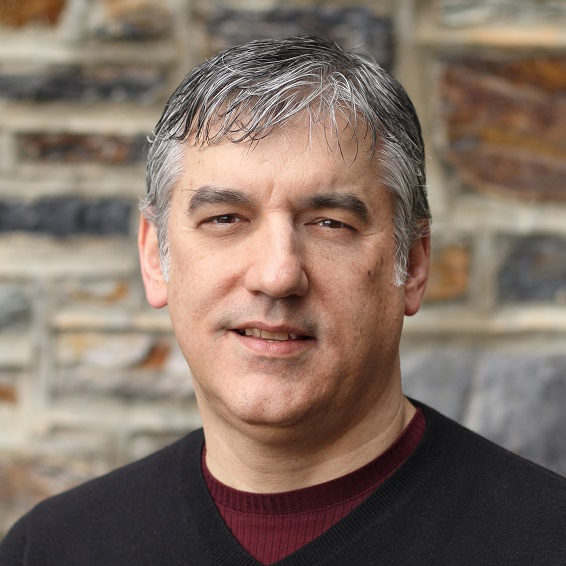
\includegraphics[height=2.1cm]{imgs/members/Chris.jpg}\\Christopher R Monroe};
        \node[align=center,below,font=\tiny] at (0, 0)
        {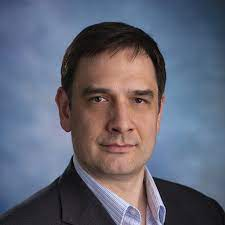
\includegraphics[height=2.1cm]{imgs/members/Alex.jpg}\\Alexander Kozhanov};
        \node[align=center,below,font=\tiny] at (3, 0)
        {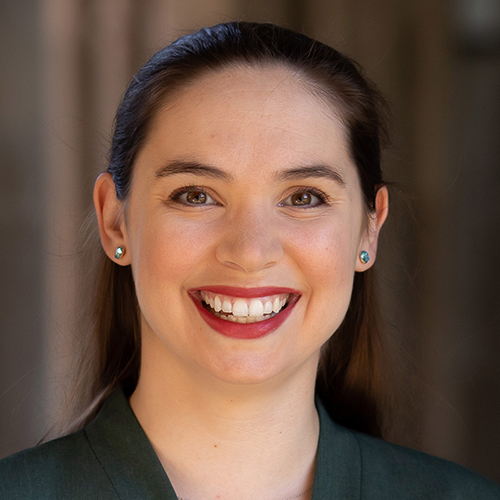
\includegraphics[height=2.1cm]{imgs/members/Crystal.jpg}\\Crystal Noel};

        \shadedraw[inner color=gray,outer color=blue!40!white,path fading = glow2 fading] (-5.8,0.05-3) rectangle (5.8,0.15-3);

        \node[align=center,below,font=\tiny] at (-4.2, -3)
        {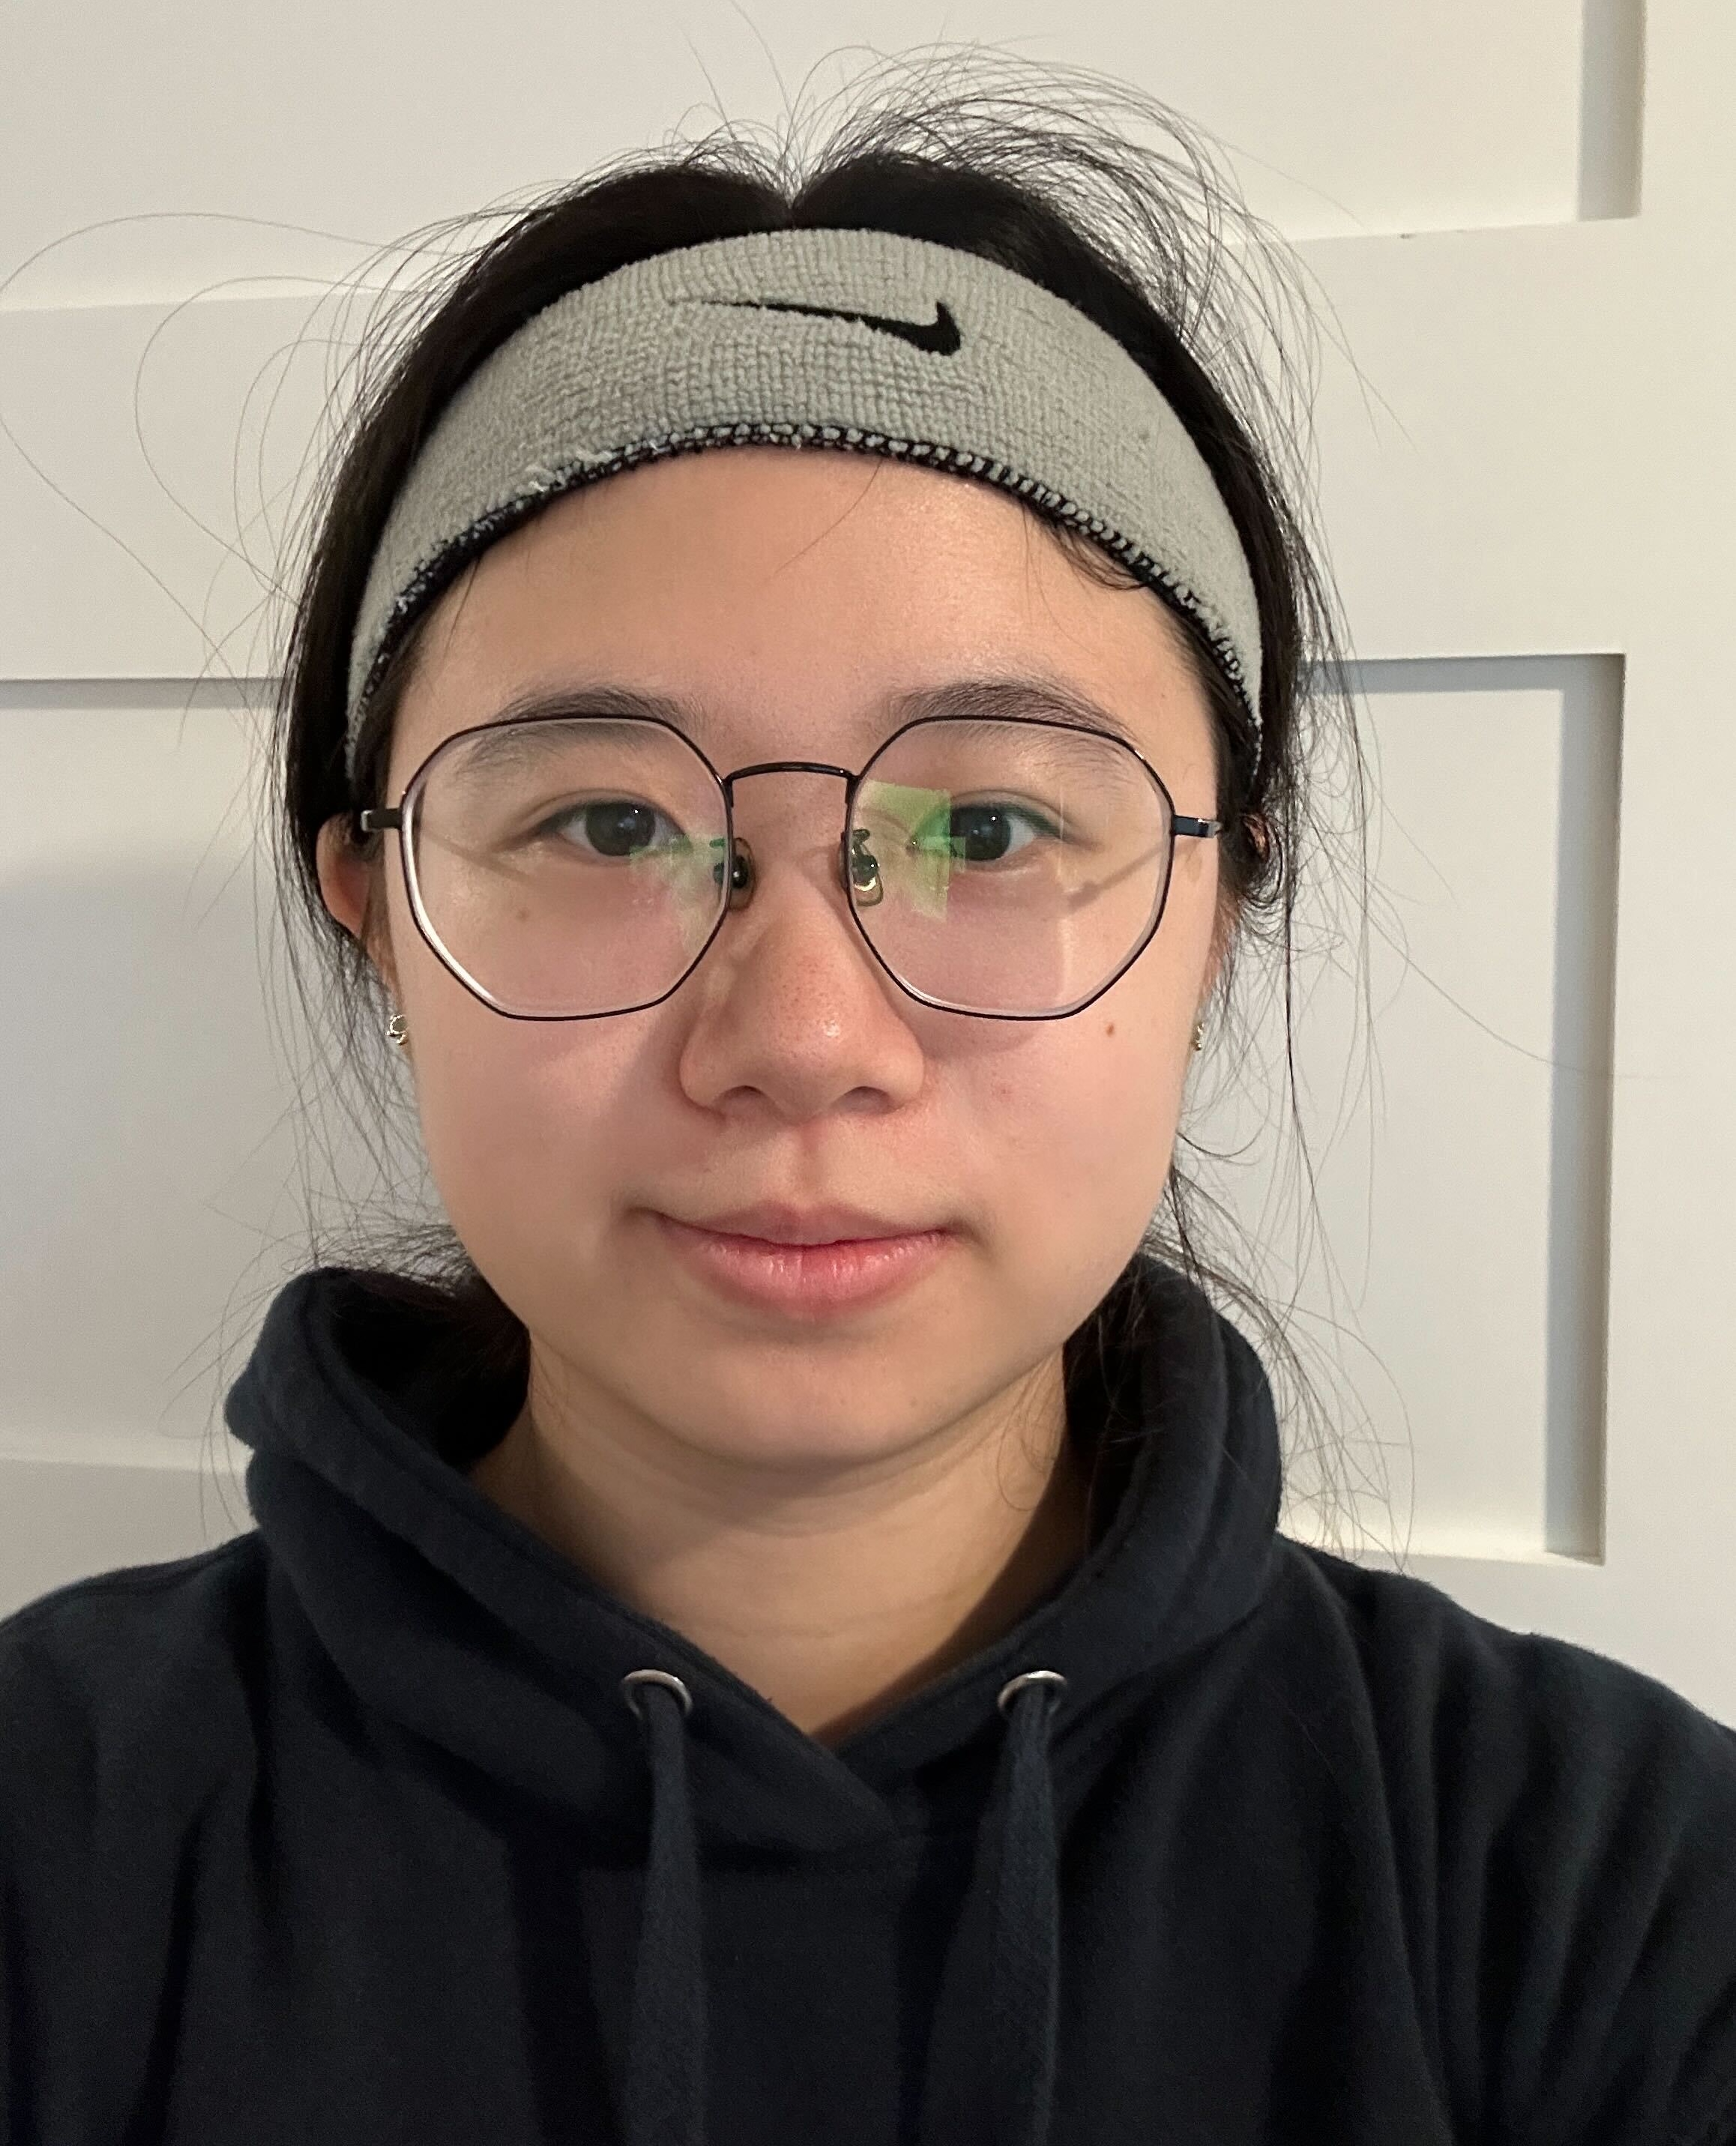
\includegraphics[height=2.1cm]{imgs/members/Keqin.jpg}\\Keqin Yan};
        \node[align=center,below,font=\tiny] at (-1.4, -3)
        {\includegraphics[height=2.1cm]{imgs/members/Vivian.png}\\Vivian Zhang};
        \node[align=center,below,font=\tiny] at (1.4, -3)
        {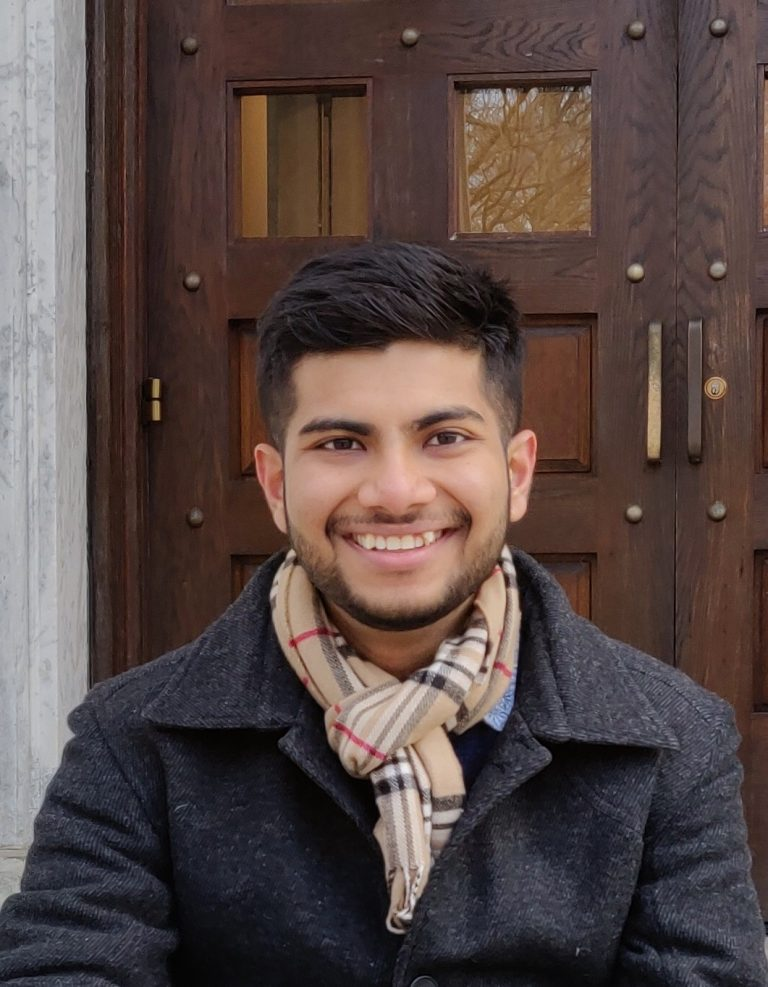
\includegraphics[height=2.1cm]{imgs/members/Debo.jpg}\\Debopriyo Biswas};
        \node[align=center,below,font=\tiny] at (4.2, -3)
        {\includegraphics[height=2.1cm]{imgs/members/Bahaa.jpg}\\Bahaa Harraz};
      \end{tikzpicture}
    \end{center}
  \end{frame}
}

\begin{frame}{}
\end{frame}

\end{document}
